%\documentclass[UTF8]{ctexart}
\documentclass{article}
\usepackage{geometry}
\usepackage{fancyhdr}
\usepackage{verbatim}
\usepackage{enumerate}
\usepackage{graphicx}
\usepackage{subfigure}
\usepackage[colorlinks,linkcolor=blue]{hyperref}
\usepackage{listings}
\usepackage{fontspec}
\setmonofont{Consolas}
\usepackage{color}
\usepackage{xcolor}
\graphicspath{{./Images/}}

\geometry{papersize={210mm,297mm}}
\geometry{left=2.5cm,right=2.5cm,top=2.5cm,bottom=2.5cm}

\setlength{\headheight}{13pt}

\title{SlopeCraft v3.6 UserGuide}
\author{TokiNoBug}
\date{\today}

\begin{comment}
\pagestyle{fancy}

\lhead{\author}
\chead{\title}
\rhead{\date}

\lfoot{}
\cfoot{\thepage}
\rfoot{}

\renewcommand{\headrulewidth}{0.4pt}
\renewcommand{\headwidth}{\textwidth}
\renewcommand{\footrulewidth}{0pt}

\end{comment}

\begin{document}
    \maketitle
    %%%%%%%%%%%%%%%%%%%%%%%
    % Page1
    %%%%%%%%%%%%%%%%%%%%%%%
    SlopeCraft is such a great update that the whole software is rewritten again with Many hardcore functions implemented and lots of bugs fixed. In this version, lossy compression is added to compress total height of a 3D map to almost any arbitrary value, which entirely sloves the problem that 3D map often got higher than the world. Also, glassbridge is added in order to assitant player when building.
    
    Besides, ui is slightly changed. Since the last tutorial is for v3.1, it's necessary to write a new user guide.

    By the way, this tutorial is not a fool-type one, only those must be introduced are introduced and those must be underlined are underlined. If any question, view a previous tutorial.

    %%%%%%%%%%%%%%%%%%%%%%%
    % Page2
    %%%%%%%%%%%%%%%%%%%%%%%
    \pagebreak
    \section{Update Summary}
    \paragraph{New Contents}

    \textbf{SlopeCraftL3.dll}——The kernel of SlopeCraft is developed into a dynamic linked library through a interface class, including core functions of 3d, flat, file-only and wall maps. Theoretically, this lib can be called by not only C++ but also Java and Python and so on.(When it comes to other languages, one more layer of interface might be required). Future plugins will have one more choice.

    \paragraph{New Functions}
    \begin{enumerate}
        \item The 61th basecolor
        \item Intelligent lossy compression
        \item Glassbridge construction——\textbf{Easy to build 3d maps}
        \item Fireproof and enderman-proof——cover vulnerable blocks with glass.
        \item Export as .NBT format——Minecraft structure block format.
        \item All kinds of \textbf{Upper slabs} to blocklist.
        \item Customizable blocklist——add any block if you like.
        \item Preview map when constructing 3d structure——\textbf{Lossy compression may edit it slightly}
        \item Check for updates and report bugs——by subject to \href{https://github.com/ToKiNoBug/SlopeCraft}{repository on GitHub}.
        \item More complete error-reporing function.
        \item Reset language automatically when starting——if Chinese isn't found in system language, English instead.
        \item settings.json——config files for starting.
        \item New map type: wall maps——kind of weird but requested for many times.
    \end{enumerate}
    \paragraph{Bug Fixed}
    \begin{enumerate}
        \item Fixed the bug that may colors can't be disabled.
    \end{enumerate}
    \paragraph{Optimization and Other Changes}
    \begin{enumerate}        
        \item Optimized the performance of converting and constructing glassbridge.
        \item Deleted unnecessary \textbf{Confirm} buttons. Less opeartions required now.
        \item Progessbars are no longer in busy state when waitting for user's operation. More suited for users now.
    \end{enumerate}

    \pagebreak
    %%%%%%%%%%%%%%%%%%%%%%%
    % Page3
    %%%%%%%%%%%%%%%%%%%%%%%
    \section{Junior Tutorial}
    \subsection{Import Image}
    From the previous tutorial to now, the greatest change is still a new button \textbf{Settings}, which is used to process transparent pixels better.
 
    Click \textbf{Settings} and you will see a subwindow as figure \ref*{SetTPS}.

    \begin{figure}[htbp]
        \centering
        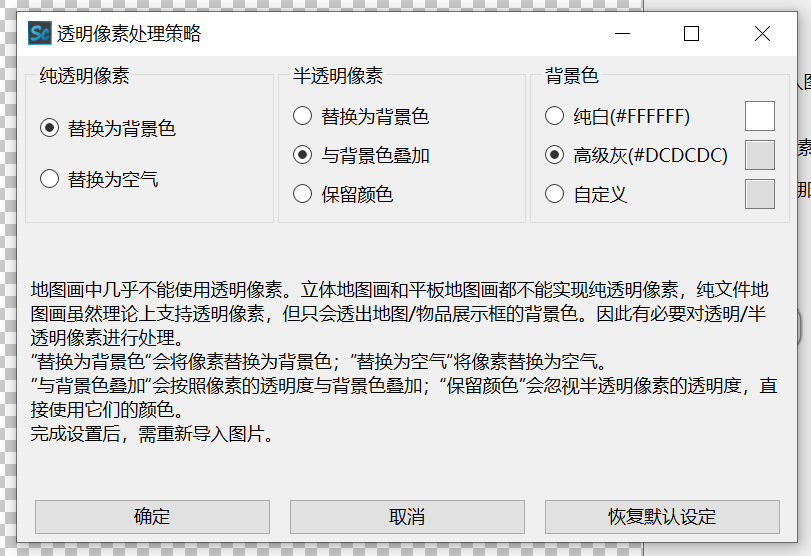
\includegraphics[width=15cm]{Img1_TPS.png}
        \caption{Subwindow to set transparence processing strategy}
        \label{SetTPS}
    \end{figure}
    
    \textbf{Note: If you want to import a image with transparency under custom transparency processing strategy, you must set the strategy first and then import you image! Otherwise the image will only be preprocessed by the default strategy! If you set the strategy after having your image imported, import you image again.}

    We have various method to deal with full-transparent pixels(alpha=0) and semitransparent pixels(alpha>0). The former are either replaced with background color or air block, while the latter have 3 choices: to be replaced with background color, to be composed with background color, or to be taken as non-transparent pixel by ignoring its alpha channel. Besides, the background color is also customizable. In default it's light gray.

    Please note that each \textbf{pixel corresponds to a block in map}. Since the width and height are recommended to be any \textbf{multiple of 128 pixels}, you should better cut and scale you image before importing into SlopeCraft.(Recommended but not forced) This preprocessing should be done by user instead of software, so I don't and won't implement such function in SlopeCraft. As a result, there is not any resizing or scaling operation in SlopeCraft, \textbf{each pixel} shall be reflected faithfully.

    \subsection{Set Map Type}
    The only modification is that a new kind of map (wall maps) is added. You just need to choose the right map type and game version following the description on ui, then turn to the next page.

    The 61th base color: GLOWING\_LICHEN is complemented to the blocklist page. Actually it was already added in Minecraft v1.17 but I left it in SlopeCraft v3.5.1.

    The logic of block list: a disabled checkbox or radiobutton mean locked or unchangeable, for example, basecolor 0(air) must be enabled. SlopeCraft requires that each basecolor must have a block eventhough the basecolor is disabled. Thus, if a basecolor has only one available block, that single radiobutton will fixed.
    
    If a block's version is later than the game version, is will also be disabled. Note that not all block can be used in wall maps, like iron pressure plate and glowing lichen. In such condition, it's not only properties of basecolors and maps themselves but also your selected blocks that restrict your available color count.

    \subsection{Color Convertion}
    There's no modification on the page of convertion. Just operate like before.
    
    First, select a converting algorithm, then set whether to enable dithering or not. Then click \textbf{Convert}, after the convertion is finished, export in the way you want.

    The 6 converting algorithms respectively correspond to 6 different color difference formulations. Among them, RGB+ is best recommended, RGB and XYZ have best speed while Lab94 and Lab00 have releatively good effect but are slow in speed. The HSV algorithm hasn't been working well for a long time, so it's not recommended.
    
    Dithering uses Floyd-Steinberg algorithm, it tries to fit the orignal image better through mixing several similar colors.
    
    Here we take picture drawn by \href{https://t.bilibili.com/544583492149793294}{Lancet\_Corgi} as an instance(Thanks to Lancet\_Corgi, here's \href{https://space.bilibili.com/37171000}{his homepage on BiliBili})
    
    \begin{figure}[htbp]
        %\addtocounter{figure}{-1}
        \centering
        \setcounter{subfigure}{0}
        \subfigure[Before Convertion]{
            \begin{minipage}[t]{7cm}
                \centering
                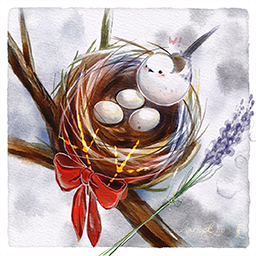
\includegraphics[width=6cm]{Img3_Raw.png}                
                \label{ruby_raw}
            \end{minipage}
        }
        \subfigure[After Convertion]{
            \begin{minipage}[t]{7cm}
                \centering
                
\includegraphics[width=6cm]{Img4_Converted.png}
                %\caption{转化后}
                \label{ruby_converted}
            \end{minipage}
        }
        \caption{Convert using RGB+(dithering disabled)}
    \end{figure}
    
    \subsection{Export 3D structure}
    If you hope to save the map in \textbf{.Litematic}(for Litematica mod) or \textbf{.nbt}(for Minecraft strcuture block) format, you should click \textbf{Build 3D} and then \textbf{Export}. When finished building, SlopeCraft will send you a preview window where you can see the material list and map.

    \begin{figure}[htbp]
        \centering
        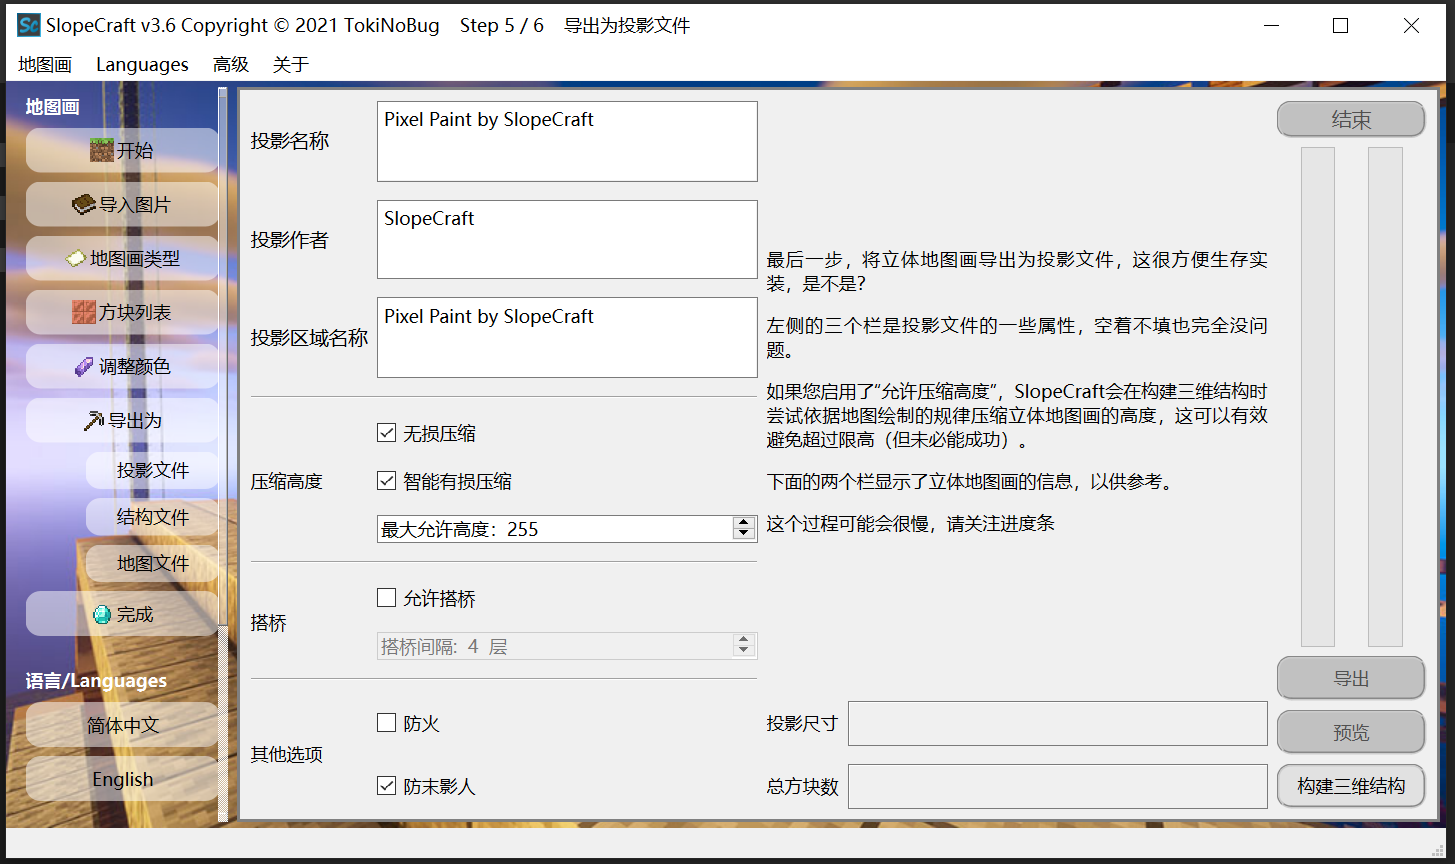
\includegraphics[width=15cm]{Img2_Export3D.png}
        \caption{Interface of Exporing 3D}
    \end{figure}

    In this interface, \textbf{Intelligent Lossy Compress} and \textbf{Construct Glass Bridge} are added. And some other options like \textbf{Fire Proof} and \textbf{Enderman Proof} are added. A new sub progress bar is used to show the progress of lossy compression and construction of glass bridge.
        
    \subsubsection{Compression}
    Simply put, lossless compression is to compress the total height of 3D map at the cost of consecutiveness while \textbf{keeping colors of each pixel strictly unchanged}. It's a really rigorous restriction so it may fail to reach your expectation. It's no exaggeration to say that some images are mathematically uncompressable, like full-white parts. Then new compress technology is required: intelligent lossy compression.

    Different with the lossless one, lossy compression compress by \textbf{slightly modifying some pixel}, to make the total height no greater than the maximum allowed height(MAH) which is assigned by you. Genetic algorithm, which belongs to swarm intelligence, is employed to implement lossy compression. So you can see it's a speacial part of SlopeCraft with most technical content. The MAH should be no less than 14, otherwise your 3D map still have some probability of failing to be compressed.

    In general, the less MAH is, the more quality loss in your map. For example, is this map is made into a 3D map, its height will be 255. Now we compress it with both lossy and lossless algorithm. Firgue \ref*{ruby_max100} shows the result when MAH=100, and \ref*{ruby_max20} shows when MAH=20.

    \begin{figure}[htbp]
        \centering
        \subfigure[MAH=100]{
            \begin{minipage}[t]{7cm}            
                \centering
                
\includegraphics[width=6cm]{Img6_Compressed_100.png}
                \label{ruby_max100}
            \end{minipage}
        }
        \subfigure[MAH=20]{
            \begin{minipage}[t]{7cm}
                \centering
                
\includegraphics[width=6cm]{Img5_Compressed_20.png}
                \label{ruby_max20}
            \end{minipage}
        }
        \caption{MAH's effect to picture quality}
    \end{figure}

    There's no obvious difference before and after the compression. But you can still find that some gray dots appear on the left and right side. You can learn that the number of gray dots has a negative relation with MAH. Otherwise, as genetic algorithm is a stochastic optimizing algorithm, there's some randomness in which pixel will be modified and regular pattern won't appear.

    Lossy and lossless compression can be used either together or respectively. But in general, if you have already enabled lossy one, there's no way to disable the lossless one. Lossy compression without lossless will make a lot more pixels modified, bringing more quality loss, while the lossless counterpart make the compression be finished with less pixel modified and less quality loss.
    
    You can choose these options with flat map or wall map, but they \textbf{won't take any result}.

    \subsubsection{Construct the Glass Bridge}
    Each horizontal slice 3D map consists of seperated blocks, which is really hard to build. Connecting these blocks will obviously make a map easier to be built. Glassbridge is what we used to connect these blocks to form a pathway to assist players.
    
    It's definatly that the glass bridge will lead to more glass consumption, so it's deprecated to construct it in each layer of 3D map. In default, SlopeCraft constructs once in each 5 layers, and that interval can be modified. A too large interval will decrease the effect while a too small interval is a waste of glass.
    
    For any details about compression and glass bridge, read \href{https://github.com/ToKiNoBug/SlopeCraftTutorial/blob/main/BasicPrinciple/Principle%20of%20map%20pixel%20arts.md}{Principle of Map Arts}.

    \href{https://github.com/AbrasiveBoar902}{AbrasiveBoar902} made great contributions to the performance of constructing glass bridge, sincere thanks to AbrasiveBoar902.

    \subsubsection{Fire Proof / Enderman Proof}
    We can learn by name that these functions is added to protect burnable blocks and prevent enderman from stealing blocks in map. The detailed method is to conver every exposed surfaces of these blocks with glass blocks, and it does work. On the other hand it consumes a large amount of glass blocks.

    \subsubsection{Export}
    There are 2 formats supported currently, \textbf{*.Litematic} and \textbf{*.nbt}.

    \begin{figure}[htbp]
        \centering
        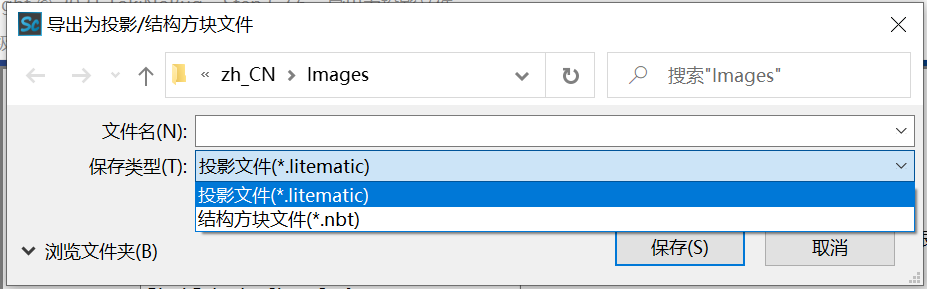
\includegraphics[width=15cm]{Img7_SelectFormat.png}
        \caption{Set Export Format}
        \label{setExport3DFormat}
    \end{figure}

    If you hope to save as \textbf{*.nbt} format, it's required to select the correct suffix, like figure \ref*{setExport3DFormat}.

    \subsection{Export as File-Only Map}
    File-only maps have few change compared to previous versions.

    File name of a map data file is like map\_i.dat, where i is an integer no less than 0, like map\_3.dat. \textbf{i is the sequence number of this map data file. Sequence number is the unqiue label of a map data file in Minecraft.} In normal conditons, your exported map data files shouldn't cover any unrelated counterparts, so be careful when setting the beginning sequence number.

    In Minecraft, pressing F3+h will enable you to learn details about an item, including map id, which is the sequence number of a map data file. Figure \ref*{mapItem} shows a map item of map\_6.dat.
   \begin{figure}[htbp]
       \centering
       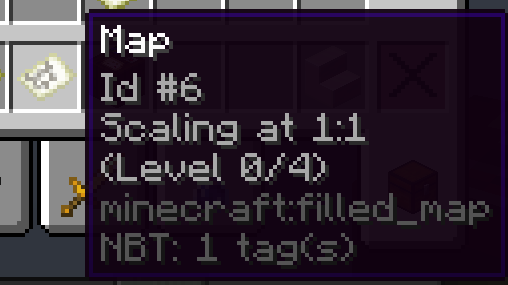
\includegraphics[height=4cm]{Img8_MapItem.png}
       \caption{Map item and map sequence number}
       \label{mapItem}
   \end{figure}

   \begin{itemize}
       \item Get map using /give command:
       
       The beginning sequence number can be set arbitarary as soon as no unreleated map will be covered.
       \begin{enumerate}
           \item 1.12 command: /give @s filled\_map 1 i
           \item 1.13+ command: /give @s filled\_map\{map:i\}
       \end{enumerate}
       \item If you want to simply replace map data files instead of using commands:
       \begin{enumerate}
           \item Create n map items correspond to your image where n is the map count, it's 4 in this instance.
           \item Press F3+H to check the map sequence number of map items you've just created, their sequence numbers should be a\textasciitilde(a+n-1), n in total.
           \item Close Minecraft and fill the value of a in the \textbf{Beginning Sequence Number} branket.
           \item Click export and then select data folder under you save. SlopeCraft will replace these map data files. 
           \item Close SlopeCraft and start Minecraft, these map items will be replaced with map pixel arts successfully.
           \item If you are afraid of your misoperation which may lead to unreleated map being covered, you can create a temporary folder and then selected when exporting. Repleace the map data files you want to replace after you're sure that no error occurres.
       \end{enumerate}
   \end{itemize}
   
   \pagebreak
   \section{Advanced Functions}
   Basical function is enough if you just want to use SlopeCraft simply. However, if you want to customize something, you'd better have a look at this section. Using advanced functions usually requires understanding of map arts' principles. It's strongly recommended to read \href{https://github.com/ToKiNoBug/SlopeCraftTutorial/blob/main/BasicPrinciple/Principle%20of%20map%20pixel%20arts.md}{Principle of map pixel arts}.

   \subsection{Customize blocklist}
   If you aren't satisfyed with default blocks, which means that you hope to add other vanilla blocks or mod-blocks, this section will tell you what to do.
   
   \subsubsection{Pre-informations}
   You must master following information first:

   \begin{enumerate}
       \item \textbf{Complete} id of this block, including \textbf{namespace prefix} and \textbf{all block properties}.
       
       For instance, waxed copper slab:
       
       minecraft:waxed\_copper\_slab[type=top,waterlogged=false]

       Here minecraft: is the namespace prefix of vanilla blocks, contents in the brackets are all block properties. For safety reason, you should set a value for every block properties.

       \item The earliest Minecraft version when this block is added.

       SlopeCraft assigned the following numbers as references of several Minecraft versions:
       \begin{table}[h]
        \centering
        \caption{Numbers and versions}
        \label{VerAndRealVer}
        \begin{tabular}{cc}\hline
            Number & Version \\ \hline
            0 & Earlier than 1.12 \\
            12 & 1.12 \\
            13 & 1.13 \\
            14 & 1.14 \\
            15 & 1.15 \\
            16 & 1.16 \\
            17 & 1.17 \\
            255 & Future version \\
            \hline            
        \end{tabular}
       \end{table}

   Usually you shouldn't use 255, it's just a reserved value. If you insist to do so, then everyting will be undefined features ---- I don't know what will happen.

   \item Block id in 1.12.
   
   This property is added simply because a great number of block ids changed from 1.12 to 1.13. If your block doesn't exist in 1.12, or its id kept unchanged, you can fill in an empty string.
   
   \item Base color of this block.
   
   Perhaps the most error prone property, but also the extremely and most important one. For vanilla blocks, view \href{https://minecraft.fandom.com/wiki/Map_item_format}{Minecraft Wiki}. For mod-blocks, measure the basecolor by yourself or ask the mod developer. Asking me will never take effort.
   
   If you don't understand what basecolor is, go to read \href{https://github.com/ToKiNoBug/SlopeCraftTutorial/blob/main/BasicPrinciple/Principle%20of%20map%20pixel%20arts.md}{Principle of map pixel arts}.

   \item Chinese name of block (arbitrary value if you don't speak Chinese).
   \item English name of block
   \item Whether another block is required under this block
   \item Whether the block glows
   \item Whether the block is burnable
   \item Whether the block can be stolen by enderman.
   \item Whether the block is suitable for wall maps(for instance, water and iron pressure plate is not suitable)
   \item Texture image of this block (16*16px png is suggested)  
   \end{enumerate}

   \subsubsection{Blocks and Blocklists}
   SlopeCraft stores blocklists in json format, while corresponding images are stored in FixedBlocks and CustomBlocks directories.
   
   There are two blocklists: fixed blocklist and cutsom blocklist. The former provides fundemental blocks which are stored in \textbf{FixedBlocks.json}(corresponding images in \textbf{FixedBlocks} directory), ensuring that each basecolor has at least one block. Although blocklists are determined at runtime, you \textbf{shouldn't modify the fixed blocklist}.
   
   The other blocklist is stored in \textbf{CustomBlocks.json}(corresponding images in \textbf{CustomBlocks} directory), this is where you add your custom blocks. Some slabs have been already written for instances.
   
   Each block has the following properties:
   \begin{table}[h]
    \centering
    \caption{Block properties}
    \begin{tabular}{ccccc}
        \hline
        Property & Type & Is compulsory & Default value & Notes  \\ \hline
        baseColor & byte & Yes & & Basecolor of the block \\
        id & string & Yes & & Complete block id\\
        version & byte & Yes & & Earliest version of the block \\
        nameZH & string & Yes & & Chinese name of the block \\
        nameEN & string & Yes & & English name of the block \\
        icon & string & Yes & & Filename of related image file \\
        idOld & string & No & Empty string & Block id in 1.12 \\
        needGlass & bool & No & false & If the block needs a block below \\
        isGlowing & bool & No & false & It the block emits light \\
        endermanPickable & bool & No & false & If can be picked by enderman \\
        burnable & bool & No & false & If the block is burnable \\
        wallUseable & bool & No & true & If the block is suitable for wall map \\
        \hline 
    \end{tabular}       
   \end{table}
   
   \clearpage
   Json code:
\begin{lstlisting}[language = C++, numbers=left, 
    numberstyle=\tiny,keywordstyle=\color{blue!70},
    commentstyle=\color{red!50!green!50!blue!50},frame=shadowbox,
    rulesepcolor=\color{red!20!green!20!blue!20},basicstyle=\ttfamily]
{
    "baseColor":11,
    "id":"minecraft:cobblestone_slab[type=top,waterlogged=false]",
    "nameZH":"圆石上半砖",
    "nameEN":"Cobblestone slab",
    "icon":"cobblestone.png",
    "version":0,
    "idOld":"minecraft:stone_slab[half=top,variant=cobblestone]"
}
    \end{lstlisting}
    The json code above shows block properties of a upper cobbleston slab, here's the interpretation:

    \begin{enumerate}
        \item It's basecolor is 11, same as stone block and cobblestone.
    
        \item It's block id is “minecraft:cobblestone\_slab[type=top,waterlogged=false]”, block statues in the brackets indicate that it's a upper slab and is not waterlogged.
    
        \item It's Chinese name is damaged due to the fucking encoding, and its English name is "Cobblestone slab".
    
        \item It's releated image is a png file named “cobblestone.png”, which is stored in CustomBlocks directory.
    
        \item It's earliest version is 0, which means that it's added before 1.12.
    
        \item It's block id has been changed in 1.13, so idOld shows it's old id in 1.12.

\end{enumerate}

    The json above doesn't show everything about this block, properties named needGlass, isGlowing, endermanPickable, burnable and wallUseable is set to default values. Thus, this block doesn't need to adhere to another block below, and it doesn't emit light, and enderman can't pick it, and it doesn't burn, and it is suitable for wall maps.

    \subsubsection{Do It Yourself}
    Having master informations as above, you are able to write in any block you want. Steps:

    \begin{enumerate}
        \item Make the your block's image into a 16 by 16 px png and move it into CustomBlocks directory.
        \item Fill in your block's json information into CustomBlocks.json, don't make mistake in json format!
        \item Restart SlopeCraft. If nothing goes wrong ,your block shall be added into blocklist successfully, otherwise remind the error message.
        \item Have fun to make your map pixel arts with SlopeCraft.
    \end{enumerate}

    \subsection{Test Your Blocklist}
    Most block-missing errors are caused by \textbf{WROUNG ID SPELLING}. If you imported lots of blocks, this function can help you to find and correct id mistakes.

    Testing blocklist will generate a special structure file, containing every blocks owned by every basecolors(unless the block is not useable for version reason). In the structure file, blocks are mapped in the same order as they are shown in the blocklist interface.
    
    If everything goes right, no block will be missing; otherwise it means an id mistake.
    
    \begin{figure}[htbp]
        \centering
        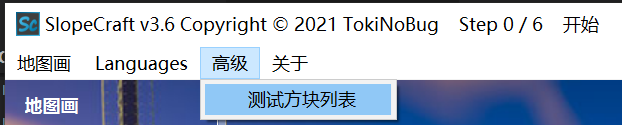
\includegraphics[width=15cm]{Img9_TestBlockList.png}
        \caption{Location of TestBlocklist}
        \label{locOfTestBlockList}
    \end{figure}

    After you have the game version selected, find and click \textbf{Test block list} under \textbf{Advanced}, then select the where to export the structure file, like figure \ref*{locOfTestBlockList}. SlopeCraft will then generate a structure like \ref*{testBlockListNBT}.

    \begin{figure}[htbp]
        \centering
        \subfigure[Left part]{
            \begin{minipage}[t]{7cm}
                \centering
                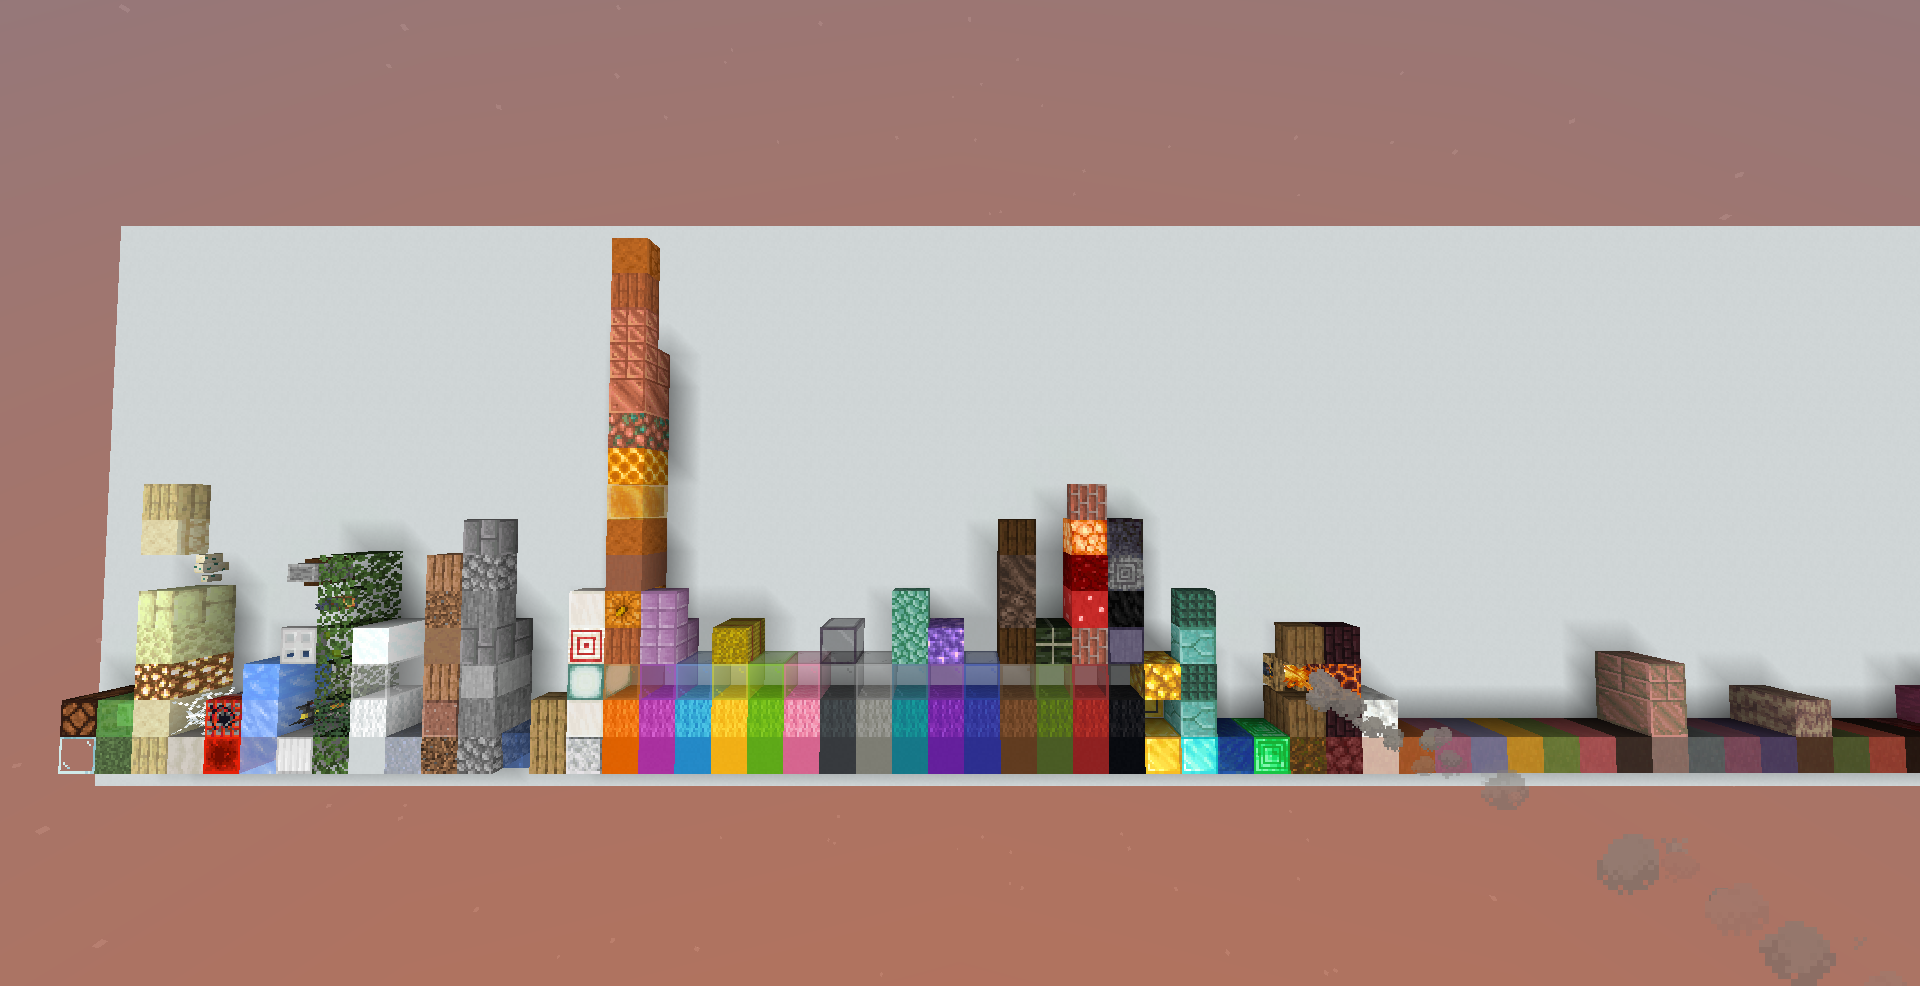
\includegraphics[width=6.5cm]{Img10_TestBlockList_Left.png}
            \end{minipage}
        }
        \subfigure[Right part]{
            \begin{minipage}[t]{7cm}
                \centering
                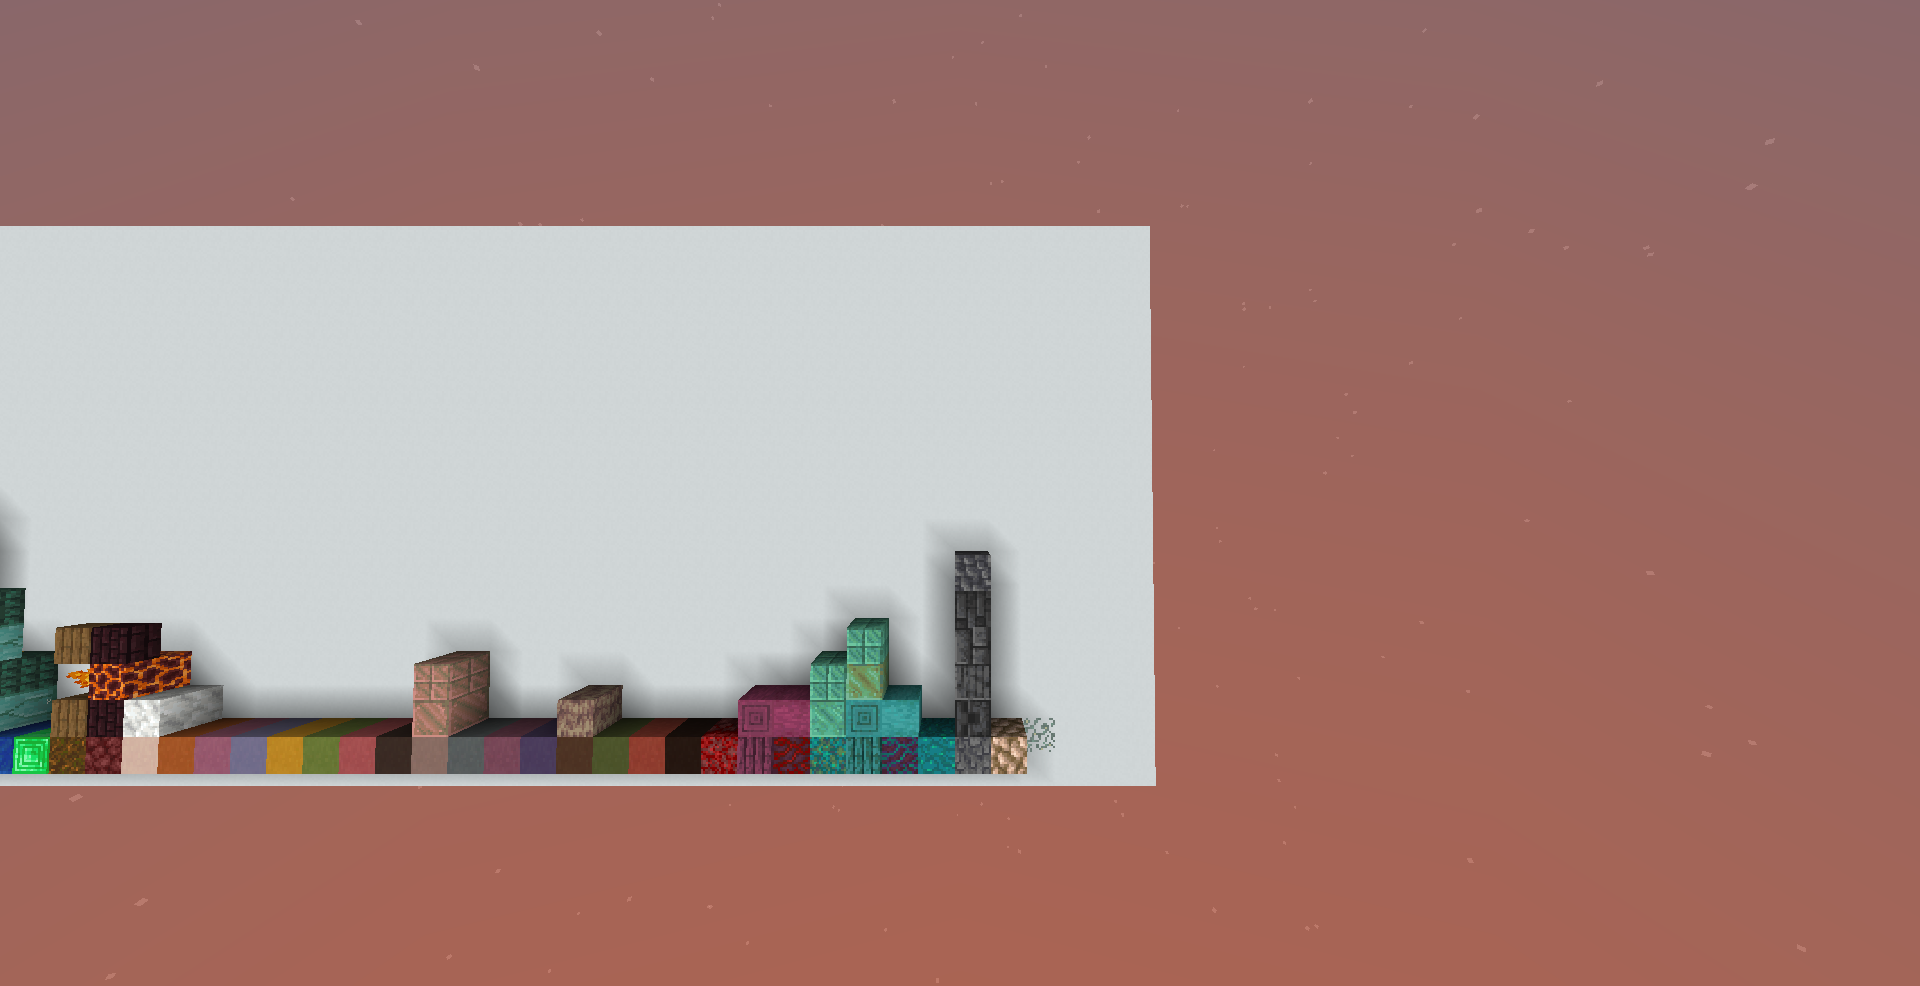
\includegraphics[width=6.5cm]{Img11_TestBlockList_Right.png}
            \end{minipage}
        }
        \caption{Test bloclist}
        \label{testBlockListNBT}
    \end{figure}

%\pagebreak
\section{Next update}
    The next version(v3.7) will have following new functions:
    \begin{enumerate}
        \item Catch up with Minecraft 1.18
        \item Batch operation to make pixel map arts
        \item Refining converted map manually
        \item ......
    \end{enumerate}

\end{document}
